\section{Group lasso}
\citep{group_lasso} introducerede en generalisering af standard lasso kaldet group lasso, som tillader, at forudbestemte grupper af prædiktorer vælges eller fravælges, således at alle prædiktorer i en specifik gruppe er enten inkluderet eller ikke inkluderet.
Afsnittet er skrevet udfra kapitel 4 i \citep{hastie} samt \citep{group_lasso}.
%I mange regressions problemer har prædiktorerne en naturlig grupperet struktur, og da foretrækkes det at alle koefficienter indenfor en gruppe er ikke-nul (eller nul) samtidig.

Betragt en lineær regressionsmodel med $J$ grupper af prædiktorer, og lad $\mathbf{z}_j$ og \(\ttheta_j\) være \(p_j \times 1\) vektorer som repræsenterer prædiktorerne i gruppe $j$ for $j=1, \ldots, J$ og deres koefficienter.
Formålet er da, at prædiktere responsvariablen $y$ baseret på prædiktorerne $\mathbf{z}_1,\ldots, \mathbf{z}_J$ \footnote{For at undgå forvirring lader vi \(\mathbf{z}_j\) og \(\ttheta_j\) betegne variablerne i gruppe \(j\) og deres koefficienter, istedet for \(\X_j\) og \(\beta_j\) som vi anvender for skalarer}.
%En lineær model for regressions funktionen $\E{Y \vert Z}$ er givet ved \(\theta_0 + \sum_{j=1}^J Z_j^T \theta_j\), hvor $\theta_j \in \R^{p_j}$ repræsenterer en gruppe af $p_j$ regressions koefficienter. 

\begin{defn}[Group lasso]
%Givet \(n\) observationer \(\cbr{ \del{y_i, z_{i,1}, z_{i,2}, \ldots, z_{i,J}}}_{i=1}^n\), da løser group lasso følgende optimeringsproblem
%Givet \(y_i, z_{i1}, z_{i2}, \ldots, z_{iJ}\) for \(i = 1, \ldots, n\), da løser group lasso følgende optimeringsproblem
Group lasso løser følgende optimeringsproblem
\begin{align}
\widehat{\ttheta}_j^{\text{group lasso}} = \argmin_{\ttheta_j \in \R^{p_j}} \cbr{\frac{1}{2} \sum_{i=1}^n \del{y_i - \sum_{j=1}^J z_{ij}^T \ttheta_j}^2 + \lambda \sum_{j=1}^J \Vert \ttheta_j \Vert_2}. \label{eq:4.5}
\end{align}
\end{defn}
For optimeringsproblemet \eqref{eq:4.5} gælder der, at
\begin{itemize}
\item Alle indgange i $\widehat{\ttheta}_j^\text{group lasso}$ vil være lig nul eller ikke-nul afhængig af \(\lambda\)
\item Når $p_j=1$, da har vi, at $\Vert \ttheta_j \Vert_2 = \vert \ttheta_j \vert$, således at alle grupper består af én prædiktor, dermed reduceres optimeringsproblemet \eqref{eq:4.5} til standard lasso.
\end{itemize}
%Figur \ref{fig:group_lasso} viser betingelsesområderne for henholdsvis group lasso og standard lasso for tre variable.
%%Vi ser at den grupperet lasso deler egenskaber med både $\ell_1$ og $\ell_2$ kuglen.
%%
%\begin{figure}[H]
%\centering
% \scalebox{0.5}{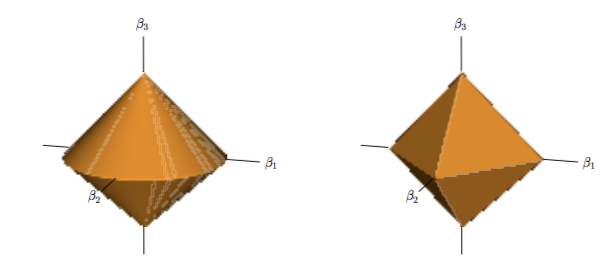
\includegraphics{fig/group_lasso.jpg}}
%\caption{Til venstre ses kuglen for group lasso i \(\R^3\) og til højre ses \(\ell_1\) kuglen.
%I dette tilfælde har vi to grupper med koefficienter \(\ttheta_1 = \del{\beta_1, \beta_2} \in \R^2\) og \(\theta_2 = \beta_3 \in \R\).}
%\label{fig:group_lasso}
%\end{figure}
%
I \eqref{eq:4.5} straffes alle grupper ligeligt, hvilket betyder, at større grupper vil have en tendens til at blive valgt.
\citep{group_lasso} anbefalede at vægte strafleddene for hver gruppe i forhold til gruppens størrelse med en faktor \(\sqrt{p_j}\).

Der findes yderligere nogle udvidelse af group lasso kaldet \textit{sparse group lasso} samt \textit{overlap group lasso}.
Sparse group lasso udfører variabeludvælgelse indenfor de valgte grupper, mens overlap group lasso tillader overlap mellem grupperne, dvs at prædiktorerne kan tilhører mere end én gruppe.
Vi vil dog kun fokuser på standard group lasso.

\subsection{Udregning af group lasso}
%
\subsubsection{Block coordinate descent}
Lad os omskrive optimeringsproblemet \eqref{eq:4.5} på matrix-vektor form
\begin{align}
\widehat{\ttheta}^{\text{group lasso}} = \argmin_{\ttheta_1, \ldots, \ttheta_J} \cbr{\frac{1}{2} \Vert \y - \sum_{j=1}^J \mathbf{Z}_{j} \ttheta_j \Vert_2^2 + \lambda \sum_{j=1}^J \Vert \ttheta_j \Vert_2}, \label{eq:4.11}
\end{align}
hvor \(\y\) er en \(n \times 1\) vektor og \(\mathbf{Z}_j\) er en \(n \times p_j\) matrix med \(j\)'te søjle \(\mathbf{z}_j\).
For dette problem er nul subgradient ligningerne givet ved
\begin{align*}
- \mathbf{Z}_{j}^T \del{\y - \sum_{\ell=1}^J \mathbf{Z}_\ell \widehat{\ttheta}^\text{group lasso}_\ell} + \lambda \widehat{\ts}_j = 0, \quad j=1,\ldots, J,
\end{align*} 
hvor $\widehat{\ts}_j $ er et element af subdifferentialet af normen $\Vert \cdot \Vert_2$ evalueret i $\widehat{\ttheta}_j^\text{group lasso}$.
Når $\widehat{\ttheta}^\text{group lasso}_j \neq 0$, har vi, at $\widehat{\ts}_j = \frac{\widehat{\ttheta}^\text{group lasso}_j}{\Vert \widehat{\ttheta}^\text{group lasso}_j \Vert_2}$, og når $\widehat{\ttheta}^\text{group lasso}_j=0$, har vi, at $\widehat{\ts}_j$ er enhver vektor, hvor $\Vert \widehat{\ts}_j \Vert_2 \leq 1$.
Block coordinate descent kan anvendes til at løse disse nul subgradient ligningerne, hvor vi løser for $\widehat{\ttheta}^\text{group lasso}_j$, mens alle block vektorer $\cbr{\widehat{\ttheta}^\text{group lasso}_k, k \neq j}$ fastholdes.
%En metode til at løse disse nul subgradient ligningerne er ved at fastholde alle block vektorer $\cbr{\widehat{\ttheta}_k, k \neq j}$, og da løse for $\widehat{\ttheta}_j$.
%Hermed udføres block coordinate descent på objektfunktionen af group lasso.
Da problemet er konveks, og strafleddet kan opdeles efter block, konvergerer algoritmen til et globalt minimum \citep{Tseng_1993}.

Lad $\cbr{\widehat{\ttheta}^\text{group lasso}_k, k \neq j}$ fastholdt, kan vi skrive
\begin{align*}
- \mathbf{Z}_{j}^T \del{\mathbf{r}_j - \mathbf{Z}_j \widehat{\ttheta}^\text{group lasso}_j} + \lambda \widehat{\ts}_j = 0,
\end{align*}
hvor $\mathbf{r}_j = \y - \sum_{k \neq j} \mathbf{Z}_k \widehat{\ttheta}_k $ er j'te partial residual.
Fra betingelserne opfyldt af subgradienten $\widehat{\ts}_j$, må vi have, at $\widehat{\ttheta}^\text{group lasso}_j =\mathbf{0}$ hvis $\Vert \mathbf{Z}_j^T \mathbf{r}_j \Vert_2 \leq \lambda$, og ellers er
\begin{align}
\widehat{\ttheta}_j^\text{group lasso} = \del{\mathbf{Z}_j^T \mathbf{Z}_j + \frac{\lambda}{\Vert \widehat{\ttheta}^\text{group lasso}_j \Vert_2} \mathbf{I}_{p_j}}^{-1} \mathbf{Z}_j^T \mathbf{r}_j. \label{eq:4.14}
\end{align}
Denne opdatering minder om løsningen af ridge regression \eqref{eq:ridge_estimator}, bortset fra at den underliggende strafparameter afhænger af $\Vert \widehat{\ttheta}^\text{group lasso}_j \Vert_2$.
Ligning \eqref{eq:4.14} har desværre ikke en lukket løsning for $\widehat{\ttheta}^\text{group lasso}_j$, medmindre at $\mathbf{Z}_j$ er ortonormal. 
I dette special tilfælde har vi, at
\begin{align*}
\widehat{\ttheta}^\text{group lasso}_j = \del{1 - \frac{\lambda}{\Vert \mathbf{Z}_j^T \mathbf{r}_j \Vert_2}}_+  \mathbf{Z}_j^T \mathbf{r}_j.
\end{align*}
%Algoritmen er stabil og vil normal nå en fornuftig konvergens tolerance indenfor få iterationer.
%De computermæssig byrde vil stige voldsomt når antallet af prædiktorer stiger.

%
%\subsection{Sparse group lasso}
%Sparse group lasso udfører variabeludvælgelse indenfor de valgte grupper, hvorimod group lasso blot udvælger grupperne.
%For at opnå denne sparsity indenfor grupperne tilføjes en \(\ell_1\) norm til standard group lasso \eqref{eq:4.11} 
%\begin{align*}
%\argmin_{\cbr{\ttheta_j \in \R^{p_j}}_{j=1}^J} \cbr{\frac{1}{2} \Vert \y - \sum_{j=1}^J \mathbf{Z}_{j} \ttheta_j \Vert_2^2 + \lambda \sum_{j=1}^J \sbr{ \del{1-\alpha} \Vert \ttheta_j \Vert_2 + \alpha \Vert \ttheta_j \Vert_1}},
%\end{align*}
%hvor \(\alpha \in \sbr{0,1}\).
%For \(\alpha = 0 \) fås group lasso og for \(\alpha = 1\) fås standard lasso.
%
%%Figur \ref{fig:sparse_group_lasso} viser betingelsesområderne for henholdsvis group lasso og sparse group lasso for tre variable.
%%Bemærk at for de to horisontale akser, da ligner betingelsesområdet det for elastisk net.
%%%
%%\begin{figure}[H]
%%\centering
%% \scalebox{0.5}{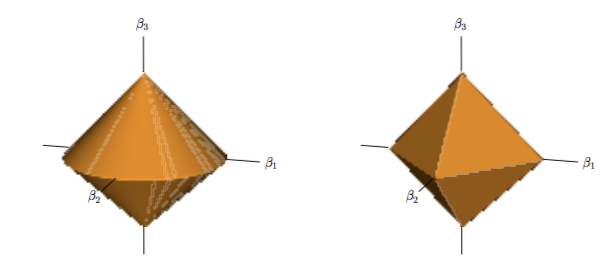
\includegraphics{fig/group_lasso.jpg}}
%%\caption{Til venstre ses kuglen for group lasso i \(\R^3\) og til højre sparse group lasso kuglen med \(\alpha = 0.5\).
%%Igen har vi to grupper med koefficienter \(\ttheta_1 = \del{\beta_1, \beta_2} \in \R^2\) og \(\theta_2 = \beta_3 \in \R\).}
%%\label{fig:sparse_group_lasso}
%%\end{figure}
%%%
%
%\subsection{Overlap group lasso}
%En anden udvidelse af group lasso tillader overlap mellem grupperne, dvs at prædiktorerne kan tilhører mere end én gruppe.

\subsubsection{LARS}
LARS algoritmen kan udvides til at løse group lasso problemet.
Vi vil dog ikke gå mere i dybden med dette, men blot referere til s. 53-55 i \citep{group_lasso}, hvor en detaljeret modificeret LARS algoritme er beskrevet.
\newpage